\chapter{ĐO ĐẠC VÀ ĐÁNH GIÁ}

\section{Một số tập dữ liệu phổ biến được sử dụng}
\subsection{Tập dữ liệu phạm vi vừa - nhỏ}
\subsubsection*{7Scenes}
Tập dữ liệu 7-Scenes \cite{6619221} bao gồm các ảnh RGB-D thuộc bảy khung cảnh khác nhau được chụp từ một máy ảnh cầm tay Kinect RGB-D ở độ phân giải 640x480. Bảy khung cảnh bap gồm: "Chess", "Fire", "Heads", "Office", "Pumpkin", "RedKitchen" và "Stairs". Với mỗi cảnh sẽ có vài chuỗi khung ảnh RGB-D. Mỗi chuỗi bao gồm khoảng từ 1000 đến 5000 khung ảnh. Mỗi khung sẽ gồm: ảnh màu, độ sâu và vị trí.
\begin{figure}[H]
	\centering
	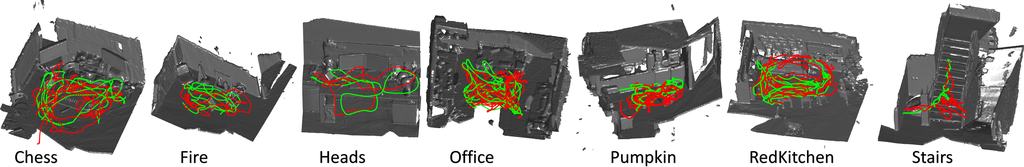
\includegraphics[width=\textwidth]{pics/Chapter2/7scenes.png}
	\caption{Minh họa tập dữ liệu 7-Scenes \cite{6619221}}
\end{figure}
\subsubsection*{Cambridge Landmark}
Tập dữ liệu Cambridge Landmarks \cite{kendall2016posenet} là một tập dữ liệu định vị thành thị bao gồm năm khung cảnh khác nhau. Các yếu tố dày đặc quan trọng như phương tiện giao thông hay người đi bộ cũng xuất hiện trong tập dữ liệu này, ngoài ra dữ liệu cũng được thu thập ở nhiều thời điểm trong ngày đại diện cho các yếu tố ánh sáng và điều kiện thời tiết khác nhau. Cambridge Landmarks được tạo ra nhờ vào việc áp dụng các kỹ thuật tái tạo kiến trúc từ chuyển động. Một chiếc điện thoại thông minh Google LG Nexus 5 được một người đi bộ trên phố sử dụng để ghi lại đoạn phim chất lượng cao cho mỗi cảnh. Mỗi đoạn phim sau đó sẽ được lấy mẫu với tần số 2Hz để trích xuất ảnh cho quy trình tái tạo kiến trúc từ chuyển động. Mỗi vị trí máy ảnh sẽ cách nhau khoảng 1m. Đây là một trong những tập dữ liệu phổ biến nhất trong việc huấn luyện và đo đạc kết quả trên các tác vụ RPR.
\begin{figure}[H]
	\centering
	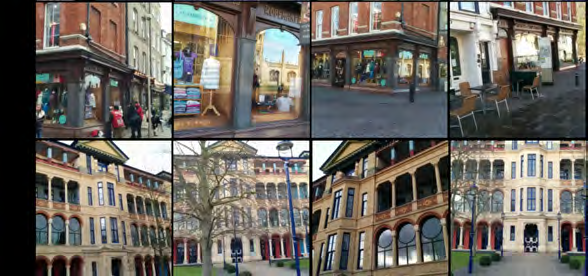
\includegraphics[width=\textwidth]{pics/Chapter2/cambridge.png}
	\caption{Minh họa tập dữ liệu Cambridge Landmarks \cite{kendall2016posenet}}
\end{figure}
\subsubsection*{Niantic Map-free Relocalization Dataset}
Tập dữ liệu Niantic Map-free Relocalization \cite{arnold2022mapfree} là một tập dữ liệu được thu thập chủ yếu để giúp ích cho phương pháp định vị Map-free \cite{arnold2022mapfree}. Tập dữ liệu bao gồm 655 cảnh bên ngoài với mỗi cảnh sẽ chứa một "địa điểm đáng chú ý" như một pho tượng, cổng, bảng hiệu,... sao cho địa điểm đó phải được xác định rõ trong một bức ảnh. Các cảnh được chia ra thành 460 cảnh phục vụ cho tác vụ huấn luyện, 65 cảnh phục vụ cho tác vụ kiểm tra quy trình huấn luyện và 130 cảnh phục vụ cho quá trình kiểm thử. Mỗi ảnh trong tập huấn luyện đều được gắn kèm vị trí tuyệt đối. Với tập kiểm thử và kiểm tra quy trình, mỗi cảnh sẽ được kèm theo một ảnh đại diện cũng như vị trí tuyệt đối tại cảnh. Ngoài ra, ma trận tham số nội tại của máy ảnh cũng được gắn kèm theo mỗi ảnh trong tập dữ liệu.
\begin{figure}[H]
	\centering
	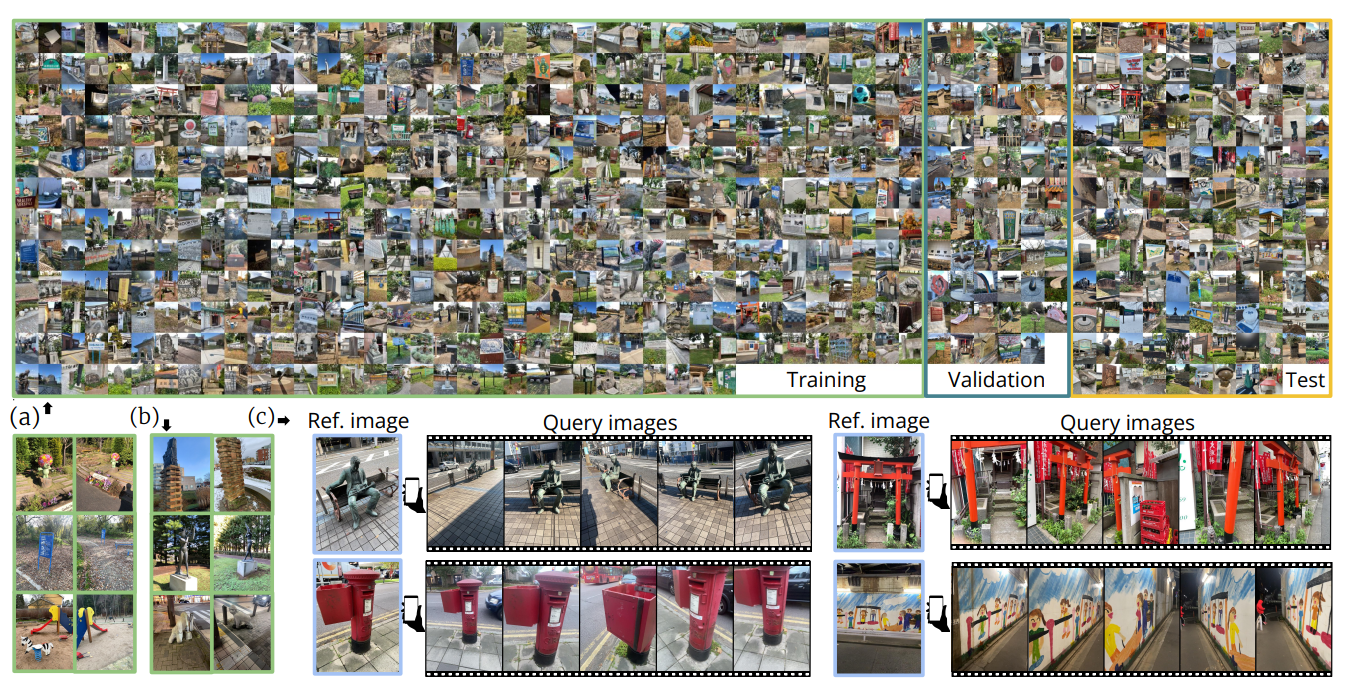
\includegraphics[width=\textwidth]{pics/Chapter2/niantic.png}
	\caption{Minh họa tập dữ liệu Niantic Map-free Relocalization \cite{arnold2022mapfree}}
\end{figure}
\subsection{Tập dữ liệu thành thị phạm vi rộng}
%\subsubsection*{Aachen Day-Night}
%Tập dữ liệu Aachen Day-Night \cite{Sattler2012ImageRF} bao gồm 14.607 ảnh được chụp với nhiều máy ảnh khác nhau bao phủ cả thành phố Aachen thuộc quốc gia Đức. Các ảnh dữ liệu được chụp ở nhiểu thời điểm trong ngày và trong năm, cụ thể là khoảng thời gian trong 2 năm. Hệ quả mang lại là tập dữ liệu bao phủ nhiều điều kiện ngoại cảnh như thời tiết, ánh sáng cũng như sự thay đổi của công trình kiến trúc trong khu vực.
%\begin{figure}[H]
%	\centering
%	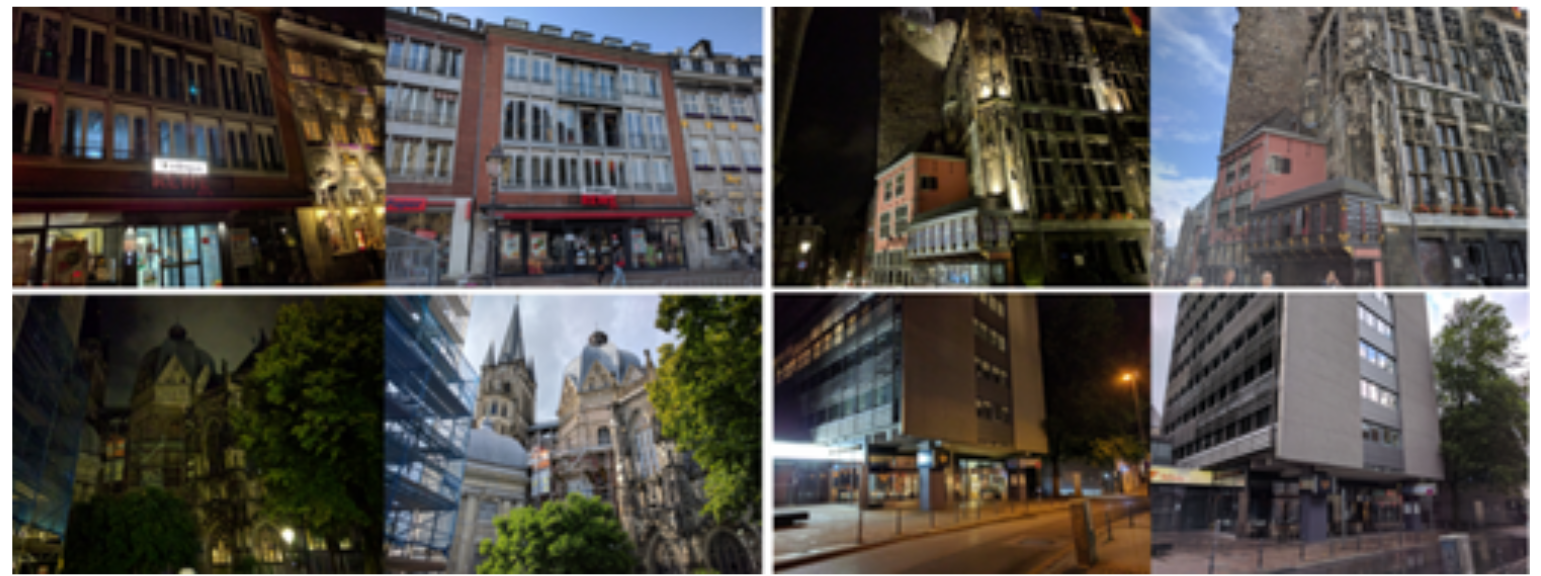
\includegraphics[width=\textwidth]{pics/Chapter2/aachen.png}
%	\caption{Minh họa tập dữ liệu Aachen Day-Night \cite{Sattler2012ImageRF}}
%\end{figure}
\subsubsection*{Pittsburgh 250k \cite{6618963}}
Tập dữ liệu Pittsburgh 250k \cite{6618963} là một tập dữ liệu tương đối rộng bao phủ thành phố Pittsburgh của Mỹ. Đây là một tập dữ liệu tương đối phổ biến trong thị giác máy tính, cụ thể là ở tác vụ nhận điện địa điểm trực quan, truy xuất ảnh và định vị trực quan.

\subsubsection*{GSV-Cities \cite{Ali_bey_2022}}
Tập dữ liệu GSV-Cities \cite{Ali_bey_2022} bao phủ một vùng địa lý cực kỳ rộng lớn với hơn 40 thành phố xuyên lục địa trong khoảng thời gian 14 năm liên tục. GSV-Cities chứa khoảng hơn 530.000 ảnh - khoảng hơn 62.000 vị trí. Mỗi vị trí sẽ có khoảng từ 4 đến 20 ảnh. Đồng thời mỗi vị trí sẽ cách nhau một khoảng ít nhất 100m.
\begin{figure}[H]
	\centering
	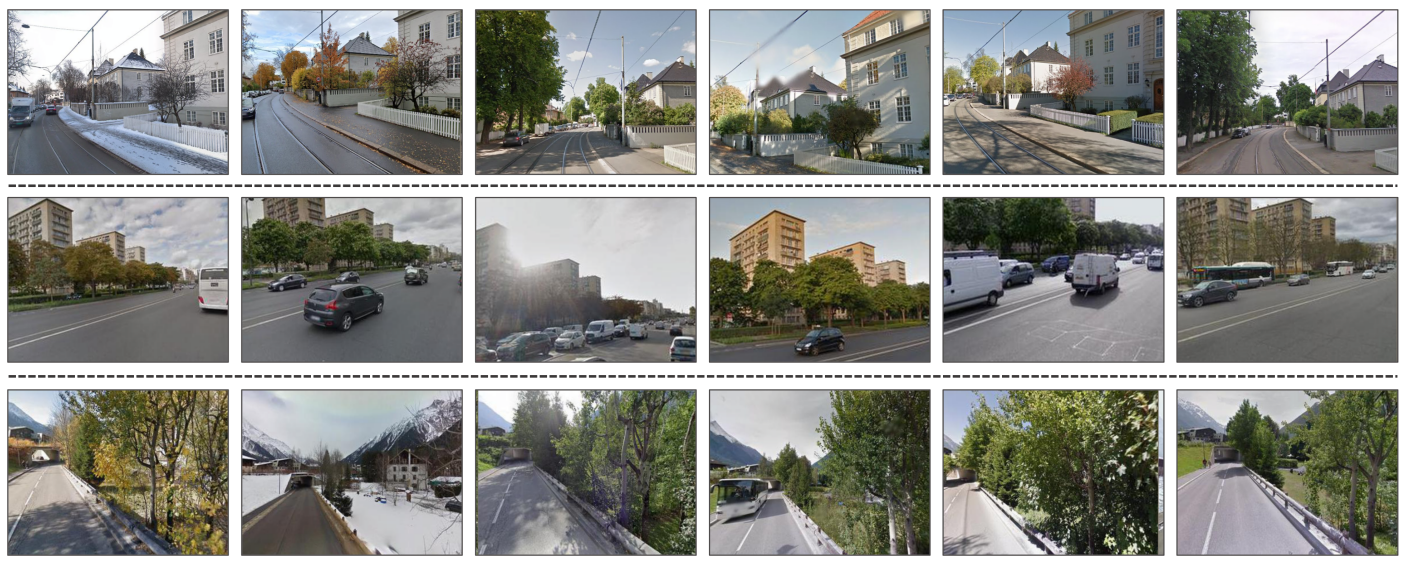
\includegraphics[width=\textwidth]{pics/Chapter2/gsv.png}
	\caption{Minh họa tập dữ liệu GSV-Cities \cite{Ali_bey_2022}}
\end{figure}

%\subsubsection*{SF-XL}
%Tập dữ liệu San Francisco Extra Large (SF-XL) \cite{berton2022rethinking} được tạo nên từ 3.43 triệu ảnh 360 độ thu thập từ kho ảnh Google Streetview. Các ảnh này sau đó được cắt ra thành 41.2 triệu ảnh. Mỗi ảnh cắt ra đều được gắn nhãn 6DoF (bao gồm cả GPS). Dữ liệu được thu thập từ năm 2009 đến năm 2021, dẫn đến việc tập dữ liệu bao phủ nhiều điều kiện ngoại cảnh như thời tiết, ánh sáng cũng như sự thay đổi của công trình kiến trúc trong khu vực.
%\begin{figure}[H]
%	\centering
%	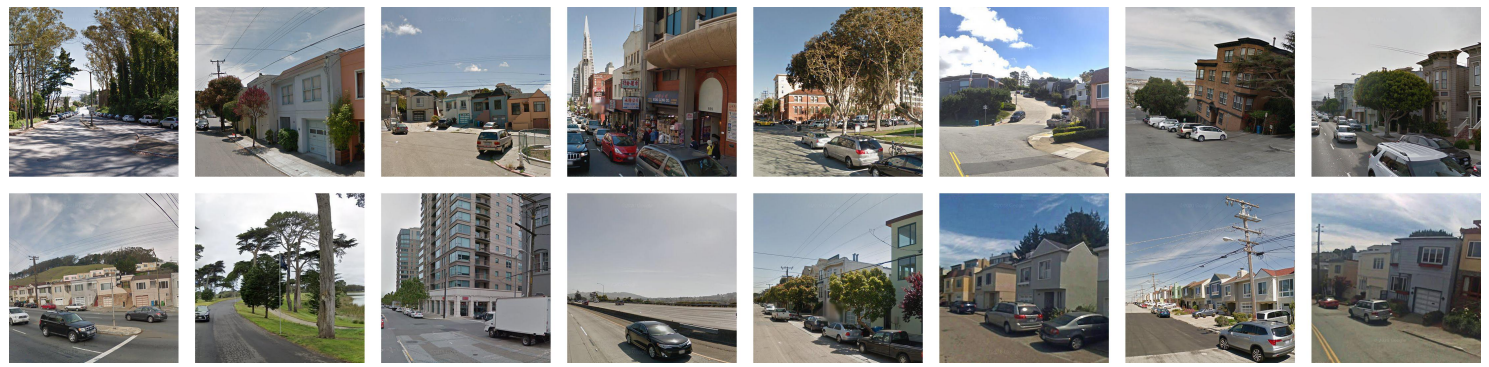
\includegraphics[width=\textwidth]{pics/Chapter2/sfxl.png}
%	\caption{Minh họa tập dữ liệu San Francisco Extra Large \cite{berton2022rethinking}}
%\end{figure}

\section{Mô hình MixVPR}
\subsection*{Mô tả quá trình thí nghiệm}

Để kiểm chứng kết quả đã được công bố trên bài báo khoa học của nhóm nghiên cứu tác giả, chúng tôi đã tiến hành chạy mô hình MixVPR \cite{alibey2023mixvpr} trên tập dữ liệu Pittsburgh 250k \cite{6618963} và tập dữ liệu Pittsburgh 30k \cite{6618963}.

Các thang đo kết quả được sử dụng trong báo cáo này sẽ là recall@k, thể hiện tỷ lệ của truy xuất thành công trên tổng số lượng truy xuất và một truy xuất hình sẽ được xem là thành công khi ảnh được truy xuất nằm trong vòng 25m xung quanh ảnh truy vấn. Để thích hợp cho việc chạy trên thiết bị cá nhân với cấu hình yếu hơn so với thiết bị của tác giả, chúng tôi đã hiệu chỉnh cài đặt kích thước mỗi batch chuyển từ 120 xuống 10, các cài đặt khác được giữ nguyên so với bài nghiên cứu.

\subsection*{Kết quả thí nghiệm}

\begin{table}[H]
	\begin{tabular}{llllllll}
		               & \textbf{R@1} & \textbf{R@5} & \textbf{R@10} & \textbf{R@15} & \textbf{R@20} & \textbf{R@50} & \textbf{R@100} \\
		Pittsburgh30k  & 91.64        & 95.55        & 96.35         & 96.99         & 97.34         & 98.25         & 98.69          \\
		Pittsburgh250k & 94.32        & 98.22        & 98.84         & 99.13         & 99.34         & 99.54         & 99.66
	\end{tabular}
\end{table}

\subsection*{Nhận xét}

Các số liệu đo đạc thu được từ thí nghiệm của chúng tôi là hoàn toàn giống với bảng kết quả đã được công bố của nhóm tác giả với recall@1 đạt 94.32\%, recall@5 đạt 98.22\%, recall@10 đạt 98.84\%. Ngoài ra, chúng tôi nhận xét rằng các cài đặt được thay đổi không ảnh hưởng đến kết quả đầu ra của mô hình mà thay vào đó chỉ ảnh hưởng đến tài nguyên thiết bị cũng như tốc độ thực thi của mô hình. Cuối cùng, với tác vụ nhận diện địa điểm trực quan, chúng tôi cho rằng các chỉ số kết quả này là đủ tốt để tiến hành sử dụng MixVPR trong mô hình kết hợp.

\section{Mô hình Map-free Relocalization}
\subsection*{Mô tả quá trình thí nghiệm}

Để kiểm chứng kết quả đã được công bố trên trang chủ của nhóm nghiên cứu tác giả công trình, chúng tôi đã tiến hành chạy quá trình hồi quy vị trí tương quan 2D - 2D của mô hình Niantic Map-free Relocalization trên tập dữ liệu kiểm thử do chính tác giả cung cấp. Cụ thể tập dữ liệu bao gồm 15.000 ảnh chia thành 130 cảnh khác nhau với mỗi cảnh bao gồm một vật thể chú ý đặt ở tâm như mô tả bài báo.

Các thang đo kết quả được sử dụng trong báo cáo này sẽ bao gồm độ lệch vị trí (m), độ lệch góc quay (độ) và sai số phản chiếu điểm 3D ảo VCRE (điểm ảnh). Các cài đặt của mô hình được giữ nguyên như trong bài nghiên cứu của tác giả.

\subsection*{Kết quả thí nghiệm}

\begin{table}[H]
	\begin{tabular}{|l|c|c|c|c|}
		\hline
		Method                                                                                                    & \multicolumn{1}{l|}{\begin{tabular}[c]{@{}l@{}}Precision \\ (Err \textless 25cm, 5°)\end{tabular}} & \multicolumn{1}{l|}{\begin{tabular}[c]{@{}l@{}}Median Trans. \\ Error (m)\end{tabular}} & \multicolumn{1}{l|}{\begin{tabular}[c]{@{}l@{}}Median Rot. \\ Error (°)\end{tabular}} & \multicolumn{1}{l|}{\begin{tabular}[c]{@{}l@{}}Median Reproj. \\ Error (px)\end{tabular}} \\ \hline
		\begin{tabular}[c]{@{}l@{}}DPT-KITTI \& SuperGlue \\ (Ess.Mat. + D.Scale) \\ (Author)\end{tabular}        & 15.4\%                                                                                             & 1.98                                                                                    & 30.5                                                                                  & 167.6                                                                                     \\ \hline
		\textbf{\begin{tabular}[c]{@{}l@{}}DPT-KITTI \& SuperGlue \\ (Ess.Mat. + D.Scale) \\ (Ours)\end{tabular}} & 15.6\%                                                                                             & 1.92                                                                                    & 26.1                                                                                  & 161.1                                                                                     \\ \hline
	\end{tabular}
	\caption{Bảng so sánh kết quả công bố và kết quả kiểm thử mô hình 2D - 2D Map-free}
\end{table}

\subsection*{Nhận xét}

Các số liệu đo đạc thu được từ thí nghiệm của chúng tôi tương đối sát với kết quả do nhóm tác giả nghiên cứu đã công bố trên trang chủ với độ lệch vị trí khoảng gần 2m và độ lệch góc quay khoảng 26 độ.

\section{Mô hình kết hợp}
\subsection*{Mô tả quá trình thí nghiệm}

Chúng tôi tiến hành tinh chỉnh mô hình MixVPR \cite{alibey2023mixvpr} với chiến lược khai phá mới mà chúng tôi đã đề xuất trên cùng tập dữ liệu GSV-Cities \cite{Ali_bey_2022}. Tuy nhiên, chúng tôi đã tiến hành chọn lọc một số thành phố đáp ứng đủ điều kiện mật độ ảnh mà nhóm đặt ra để đảm bảo rằng mỗi khu vực đều có độ đa dạng về góc nhìn. Chúng tôi chọn kích thước batch là 8 nơi với mỗi nơi gồm 16 ảnh, tức tạo thành một batch với 128 ảnh. Một lớp feature mixer được đóng băng trong quá trình tinh chỉnh. Chúng tôi tiến hành tinh chỉnh qua 5 epoch với learning rate được chỉnh về 0.0005. Các ngưỡng frustum và góc quay được đặt là 1.25 và 60 độ theo thứ tự. Các cài đặt không được nêu lên sẽ được giữ nguyên như bài báo gốc.

Chúng tôi tiến hành kiểm thử kết quả mô hình kết hợp trên các tập dữ liệu thường dùng cho hai tác vụ VPR và RPR riêng biệt: trên tập dữ liệu thành thị phạm vi rộng nhưng mật độ ảnh thưa (Pitts250k-test \cite{6618963}) và trên một tập dữ liệu kích thước vừa nhưng mật độ ảnh cao (Cambridge Landmark \cite{kendall2016posenet}).

Với tác vụ VPR, chúng tôi tiến hành đo đạc kết quả của mô hình kết hợp trước và sau khi tinh chỉnh, sau đó so sánh với các mô hình cơ sở khác đã được huấn luyện sẵn bao gồm: MixVPR gốc \cite{alibey2023mixvpr}, NetVLAD \cite{arandjelovic2016netvlad} và AnyLoc \cite{keetha2023anyloc}. Thí nghiệm được tiến hành trên tập dữ liệu Pittsburgh250k-test \cite{6618963}. Thang đo kết quả được sử dụng trong thí nghiệm này sẽ là trung bình độ lệch vị trí và góc quay với đơn vị (mét, độ) theo thứ tự.

Các mô hình sẽ vừa được so sánh với tư cách riêng lẻ vừa kết hợp với tác vụ RPR trong mô hình kết hợp của chúng tôi. Với NetVLAD \cite{arandjelovic2016netvlad}, chúng tôi sử dụng mô hình đã được huấn luyện sẵn trên tập Pittsburgh250k. Với AnyLoc \cite{keetha2023anyloc},  chúng tôi sử dụng các thiết lập mặc định như trong bài báo khoa học của nhóm nghiên cứu tác giả. Lưu ý, do mô hình RPR yêu cầu các tập dữ liệu ảnh sẽ cần phải cung cấp các thông số nội tại, chúng tôi đã sử dụng COLMAP để tính toán các tham số nội tại cho tập dữ liệu Pittsburgh250k trước khi đưa vào thí nghiệm đo đạc, các tham số này chỉ mang tính chất tham khảo và không nên áp dụng phương pháp này khi xây dựng tập dữ liệu thành thị mới.

\bgroup
\def\arraystretch{1.4}%
\setlength\tabcolsep{10 pt}
\begin{table}[H]
\centering
\begin{tabular}{|l|c|c|c|}
\hline
                                & Dim   & Med. Trans. Err & Med. Rot. Err \\ \hline
AnyLoc \cite{keetha2023anyloc}  & 12288 & 42.56           & 46.66         \\
AnyLoc + RPR (Ours)             & 12288 & 41.39           & 47.57         \\ \hline
MixVPR \cite{alibey2023mixvpr}  & 4096  & 21.82           & \textbf{36.57}\\
MixVPR + RPR (Ours)             & 4096  & {\ul 18.96}     & { \ul 39.20}         \\ \hline
NetVLAD \cite{arandjelovic2016netvlad} & 32768 & 84.88             & 47.68           \\
NetVLAD + RPR (Ours)            & 32768 & 77.39           & 48.28         \\ \hline
MixVPR + RPR (Ours)             & 4096  &\textbf{18.32}   & 39.39   \\
(fine-tuned VPR)                &       &                 &               \\ \hline
\end{tabular}
\vspace{10pt}
\caption[Kết quả định vị trực quan trên tập Pittsburgh250k-test]{Kết quả định vị trực quan trên tập Pittsburgh250k-test \cite{6618963}. Thang đo trung bình độ lệch vị trí và góc quay được áp dụng cho các mô hình được so sánh. Kết quả tốt nhất và tốt thứ nhì được đánh dấu (với in đậm/gạch dưới, theo thứ tự).}
\end{table}
\egroup

Với tác vụ RPR, chúng tôi tiến hành đo đạc kết quả của mô hình kết hợp trước và sau khi tinh chỉnh, sau đó so sánh với các mô hình cơ sở khác đã được huấn luyện sẵn bao gồm: EssNet \cite{zhou2020learn}, NC-EssNet \cite{zhou2020learn} và Relformer \cite{idan2023learning}. Đồng thời, chúng tôi cũng áp dụng các mô hình VPR được so sánh ở thí nghiệm trước lên thí nghiệm này nhằm kiểm chứng độ hiệu quả. Thí nghiệm được tiến hành trên tập dữ liệu Cambridge Landmark \cite{kendall2016posenet}. Thang đo kết quả được sử dụng trong thí nghiệm này sẽ là trung bình độ lệch vị trí và góc quay với đơn vị (mét, độ) theo thứ tự. Do trọng tâm của chúng tôi là việc áp dụng định vị trực quan lên dữ liệu chưa từng thấy, không mô hình nào trong thí nghiệm này từng được huấn luyện trên tập dữ liệu Cambridge Landmark \cite{kendall2016posenet}.

\bgroup
\def\arraystretch{1.4}%
\setlength\tabcolsep{10 pt}
\begin{table}[H]
\centering
\begin{tabular}{|l|c|c|}
\hline
                             & Median Trans. Err & Median Rot. Err \\ \hline
EssNet \cite{zhou2020learn}  & 10.40             & 85.80           \\
NC-EssNet \cite{zhou2020learn} & 7.98              & 24.40           \\
Relformer \cite{idan2023learning} & 3.35              & 10.60           \\ \hline
NetVLAD \cite{arandjelovic2016netvlad} & 3.99              & 10.03           \\
AnyLoc \cite{keetha2023anyloc} & 4.46              & 10.42           \\
MixVPR \cite{alibey2023mixvpr} & 4.04              & 7.44            \\ \hline
\textbf{MixVPR + RPR} (Ours)        & \textbf{3.17}     & \textbf{4.76}   \\
{\ul MixVPR + RPR (Ours)} & {\ul 3.19}        & {\ul 4.80}      \\ 
{(\ul fine-tuned VPR)} &  &        \\ \hline
\end{tabular}
\vspace{10pt}
\caption[Kết quả định vị trực quan trên tập Cambridge Landmark]{Kết quả định vị trực quan trên tập Cambridge Landmark \cite{kendall2016posenet}. Thang đo trung bình độ lệch vị trí và góc quay được áp dụng cho các mô hình được so sánh. Kết quả tốt nhất và tốt thứ nhì được đánh dấu (với in đậm/gạch dưới, theo thứ tự).}
\end{table}
\egroup

\subsection*{Nhận xét}

Nhận xét về kết quả đo được với tác vụ VPR trên tập dữ liệu Pittsburgh250k-test \cite{6618963}:
\begin{itemize}
	\item Áp dụng mô hình kết hợp lên các mô hình VPR giúp giảm thiểu độ lệch vị trí, nhưng lại tăng độ lệch góc quay.
	\item Mô hình tinh chỉnh của chúng tôi đạt kết quả tốt nhất về mặt độ lệch vị trí trung bình và có phần giảm thiểu vấn đề sai số góc quay của mô hình kết hợp cơ sở.
	\item Sai số lớn về góc quay ở mô hình kết hợp có thể dẫn đến bởi việc các ảnh truy xuất được từ VPR chưa đủ độ trùng lắp phù hợp để tác vụ RPR có thể hoàn thành tốt việc tính toán tư thế.
	\item Sai số lớn về góc quay còn có thể dẫn đến bởi việc mô hình cơ sở xử lý tác vụ feature matching hoạt động chưa đủ hiệu quả với các tập dữ liệu thành thị đa dạng về góc quay. Ngoài ra, các thông số nội tại máy ảnh được tạo bởi COLMAP chỉ mang tính chất tham khảo, có thể dẫn đến sai số trong quá trình hồi quy tư thế.
	\item Hiện tượng kiến trúc trùng lặp (các cảnh cách xa nhau nhưng có độ tương đồng cao về mặt hình ảnh, đặc trưng) ở tập dữ liệu Pittsburgh250k \cite{6618963} có thể dẫn đến việc truy xuất ảnh sai và từ đó hồi quy sai tư thế.
	\item Ngoài ra, nhận thấy tác vụ dự đoán độ sâu của mô hình cơ sở vẫn còn nhiều sai sót, dẫn đến các sai sót trong quy trình hồi quy tư thế của toàn mô-đun RPR.
	\begin{figure}[H]
		  \centering
		  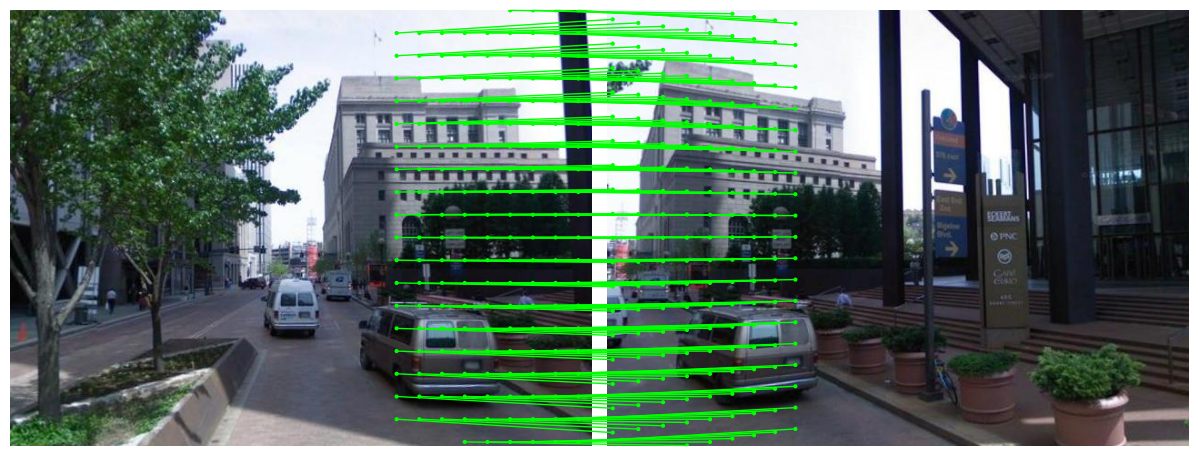
\includegraphics[width=\textwidth]{pics/Chapter3/lowoverlap_match.png}
		  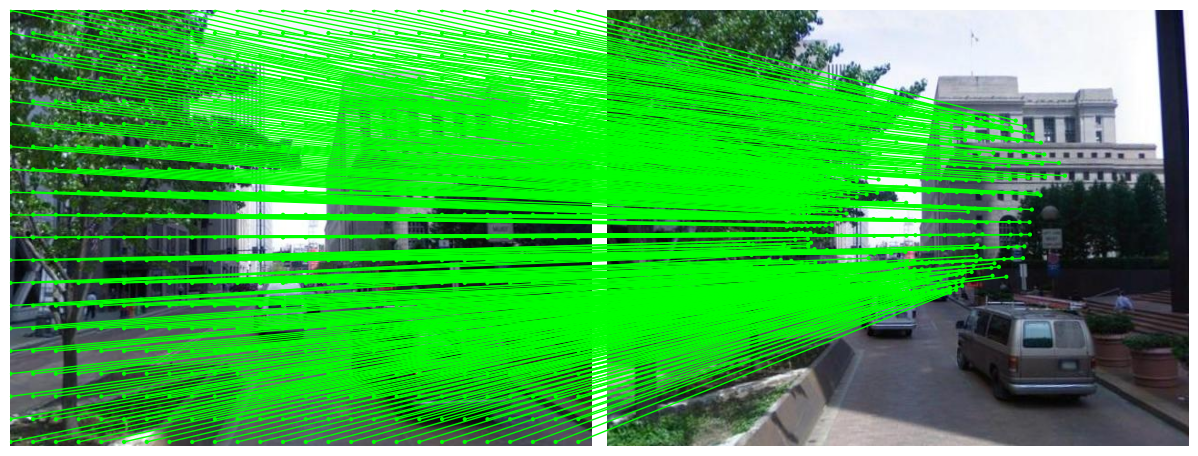
\includegraphics[width=\textwidth]{pics/Chapter3/highoverlap_match.png}
		  \caption[Ảnh matching không đúng]{Matching sai lệch do scale giữa các cặp ảnh}
	\end{figure}
\end{itemize}


Nhận xét về kết quả đo được với tác vụ RPR trên tập dữ liệu Cambridge Landmark \cite{kendall2016posenet}:
\begin{itemize}
	\item Mô hình kết hợp của chúng tôi đạt kết quả tốt nhất và tốt thứ nhì trên tập Cambridge Landmark \cite{kendall2016posenet}.
	\item Có thể giải thích kết quả trên là do: chúng tôi kết hợp độ khái quát hóa tốt của tác vụ VPR và khả năng tính toán tư thế tuyệt đối chuẩn xác của tác vụ RPR, dẫn đến việc mô hình kết hợp đạt được kết quả tốt nhất dù chưa từng được huấn luyện trên tập dữ liệu này. 
	\item Tác vụ RPR hoạt động tốt hơn khi mật độ ảnh cùng nhìn vào một địa điểm cao. Cụ thể là mô hình cơ sở feature matching sẽ được cải thiện hiệu suất khi các ảnh có độ trùng lắp cao. Ngoài ra các tham số nội tại thuộc tập dữ liệu Cambridge Landmark được cung cấp bởi tác giả, dẫn đến không có sai số thêm trong quá trình tính toán tư thế. 
	\item Các mô hình VPR tuy có độ chuẩn xác cao trong việc truy xuất ảnh nhưng lại không có khả năng tính toán được tư thế chính xác của ảnh được chụp dẫn đến kết quả có phần tệ hơn.
	\item Các mô hình RPR tuy có khả năng tính toán tốt tư thế tuyệt đối trong những tập dữ liệu vừa và nhỏ song lại có thể mắc phải tình trạng quá khớp vào tập dữ liệu huấn luyện, dẫn đến kết quả không quá khả quan.
\end{itemize}


\section{Kết luận}
Chúng tôi đã có thể đo đạc và so sánh kết quả các mô hình khác nhau với phương pháp đề xuất của nhóm. Chúng tôi rút ra được một số nhận xét tổng thể về điểm mạnh và điểm yếu cần cải thiện của giải pháp đề xuất. Trước hết, về điểm mạnh:
\begin{itemize}
	\item Mô hình kết hợp của chúng tôi kết hợp được độ tổng quát hóa cao của VPR và độ chính xác chi tiết của RPR trong tác vụ hồi quy tư thế, dẫn đến kết quả tốt hơn hết trong tác vụ RPR trên dữ liệu chưa được huấn luyện.
	\item Sử dụng mô hình cơ sở giúp giảm thiểu tài nguyên cũng như thời gian huấn luyện.
	\item Tác vụ RPR với các mô hình cơ sở giúp mô hình hoạt động tốt với nhiều tập dữ liệu hơn so với các mô hình học sâu.
\end{itemize}
Về các điểm cần cải thiện:
\begin{itemize}
	\item Việc sử dụng các mô hình cơ sở được huấn luyện sẵn tiềm ẩn nhiều rủi ro sai lệch trong các bước của mô hình, dẫn đến sai số lớn ở kết quả đầu ra.
	\item Các mô hình feature matching thường hoạt động tốt trong môi trường indoor, hoặc với một vật thể cố định nào đó thay vì toàn cảnh đô thị.
	\item Thời gian thực thi của các nhiều mô hình cơ sở sẽ làm tăng thời gian thực thi của toàn thể mô hình kết hợp.
\end{itemize}